\documentclass[12pt,letterpaper]{exam}
\usepackage[lmargin=1in,rmargin=1in,tmargin=1in,bmargin=1in]{geometry}
\usepackage{../style/exams}

% -------------------
% Course & Exam Information
% -------------------
\newcommand{\course}{MAT 107: Exam 1}
\newcommand{\term}{Winter --- 2022}
\newcommand{\examdate}{01/08/2023}
\newcommand{\timelimit}{Time Limit: `$\infty$'}

\setbool{hideans}{false} % Student: True; Instructor: False

% Logical Circuits
\usepackage{circuitikz}
\usetikzlibrary{shapes.gates.logic.US,shapes.gates.logic.IEC}

\DeclareRobustCommand{\longerleftarrow}{\DOTSB\leftarrow\joinrel\relbar\joinrel\relbar} % Long Left Arrow
\newcommand{\nim}[2]{\underset{#1}{\hspace{0.1cm}\underline{\hspace{0.2cm} \text{#2} \hspace{0.2cm}} \hspace{0.1cm}}}

%\usepackage[table,xcdraw]{xcolor} % Black Filled Cell, Load early to avoidclas

% -------------------
% Content
% -------------------
\begin{document}

\examtitle
\instructions{Write your name on the appropriate line on the exam cover sheet. This exam contains \numpages\ pages (including this cover page) and \numquestions\ questions. Check that you have every page of the exam. Answer the questions in the spaces provided on the question sheets. Be sure to answer every part of each question and show all your work. If you run out of room for an answer, continue on the back of the page --- being sure to indicate the problem number.} 
\scores
\bottomline
\newpage

% ---------
% Questions
% ---------
\begin{questions}

% Question 1
\newpage
\question[10] Construct the logic table for $P \to (\neg P \vee Q)$. \pspace

\sol \par
	\begin{table}[h]
	\centering
	\begin{tabular}{c|c||c|c||c}
	$P$ & $Q$ & $\neg P$ & $\neg P \vee Q$ & $P \to (\neg P \vee Q)$ \\ \hline
	$T$ & $T$ & $F$ & $T$ & $T$ \\
	$T$ & $F$ & $F$ & $F$ & $F$ \\
	$F$ & $T$ & $T$ & $T$ & $T$ \\
	$F$ & $F$ & $T$ & $T$ & $T$
	\end{tabular}
	\end{table}



% Question 2
\newpage
\question[10] Show that $\neg (P \to Q)$ and $P \wedge \neg Q$ are logically equivalent. \pspace

\sol \par
	\begin{table}[h]
	\centering
	\begin{tabular}{c|c||c|c||c|c}
	$P$ & $Q$ & $P \to Q$ & $\neg (P \to Q)$ & $\neg Q$ & $P \wedge \neg Q$ \\ \hline
	$T$ & $T$ & $T$ & $\mathbf{F}$ & $F$ & $\mathbf{F}$ \\
	$T$ & $F$ & $F$ & $\mathbf{T}$ & $T$ & $\mathbf{T}$ \\
	$F$ & $T$ & $T$ & $\mathbf{F}$ & $F$ & $\mathbf{F}$ \\
	$F$ & $F$ & $T$ & $\mathbf{F}$ & $T$ & $\mathbf{F}$ 
	\end{tabular}
	\end{table} \par
Because the bolded columns have the same logical outputs for the same logical inputs, we know that $\neg (P \to Q)$ and $P \wedge \neg Q$ are logically equivalent; that is, $\neg (P \to Q) \equiv P \wedge \neg Q$. Alternatively, using the fact that $P \to Q \equiv \neg P \vee Q$, we have\dots
	\[
	\neg (P \to Q) \equiv \neg (\neg P \vee Q) \equiv \neg (\neg P) \wedge \neg Q \equiv P \wedge \neg Q
	\]



% Question 3
\newpage
\question[10] Find the logical expression corresponding to the following circuit:
	\[
	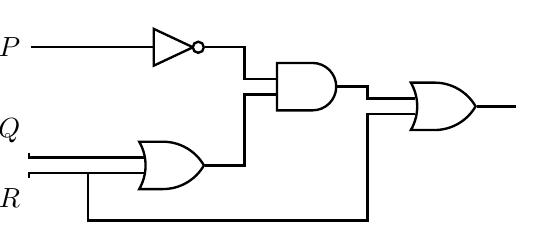
\begin{tikzpicture}
	\node (p) at (0,2) {\hspace{-0.5cm}$P$};
	\node (q) at (0,0.94) {\hspace{-0.5cm}$Q$};
	\node (r) at (0,0.091) {\hspace{-0.5cm}$R$};
	
	\node[not gate US, draw, line width= 0.03cm] at (1.75,2) (not1) {}; % Upper NOT
	\node[or gate US, draw, line width= 0.03cm] at (1.75,0.5) (or1) {}; % Lower OR
	\node[and gate US, draw, line width= 0.03cm] at (3.5,1.5) (and1) {}; % Middle AND
	\node[or gate US, draw, line width= 0.03cm] at (5.2,1.25) (or2) {}; % Right OR
	
	\draw[line width= 0.03cm] (not1.input) |- (p); % P to NOT
	\draw[line width= 0.03cm] (q) |- (or1.input 1); % Q to OR
	\draw[line width= 0.03cm] (r) |- (or1.input 2); % R to OR
	
	\draw[line width= 0.03cm] (not1.output) -- ([xshift=0.5cm]not1.output) |- (and1.input 1); % NOT to AND
	\draw[line width= 0.03cm] (or1.output) -- ([xshift=0.5cm]or1.output) |- (and1.input 2); % OR to AND
	
	\draw[line width= 0.03cm] (and1.output) -- ([xshift=0.38cm]and1.output) |- (or2.input 1); % AND to OR
	\draw[line width= 0.03cm] (0.75,0.4) -- (0.75,-0.2) -- ([xshift=3.55cm]0.75,-0.2) |- (or2.input 2); % R to OR
	\draw[line width= 0.03cm] (or2.output) -- ([xshift=0.5cm]or2.output); % OR tail
	\end{tikzpicture}
	\] \pspace

\sol We follow each wire, labeling the outputs of each circuit. 
	\[
	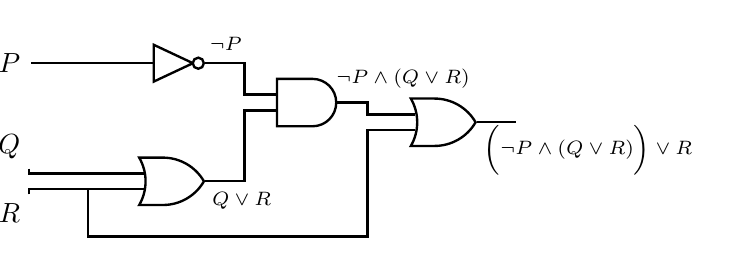
\begin{tikzpicture}
	\node (p) at (0,2) {\hspace{-0.5cm}$P$};
	\node (q) at (0,0.94) {\hspace{-0.5cm}$Q$};
	\node (r) at (0,0.091) {\hspace{-0.5cm}$R$};
	
	\node[not gate US, draw, line width= 0.03cm] at (1.75,2) (not1) {}; % Upper NOT
	\node[or gate US, draw, line width= 0.03cm] at (1.75,0.5) (or1) {}; % Lower OR
	\node[and gate US, draw, line width= 0.03cm] at (3.5,1.5) (and1) {}; % Middle AND
	\node[or gate US, draw, line width= 0.03cm] at (5.2,1.25) (or2) {}; % Right OR
	
	\draw[line width= 0.03cm] (not1.input) |- (p); % P to NOT
	\draw[line width= 0.03cm] (q) |- (or1.input 1); % Q to OR
	\draw[line width= 0.03cm] (r) |- (or1.input 2); % R to OR
	
	\draw[line width= 0.03cm] (not1.output) -- ([xshift=0.5cm]not1.output) |- (and1.input 1); % NOT to AND
	\draw[line width= 0.03cm] (or1.output) -- ([xshift=0.5cm]or1.output) |- (and1.input 2); % OR to AND
	
	\draw[line width= 0.03cm] (and1.output) -- ([xshift=0.38cm]and1.output) |- (or2.input 1); % AND to OR
	\draw[line width= 0.03cm] (0.75,0.4) -- (0.75,-0.2) -- ([xshift=3.55cm]0.75,-0.2) |- (or2.input 2); % R to OR
	\draw[line width= 0.03cm] (or2.output) -- ([xshift=0.5cm]or2.output); % OR tail
	
	\node at (2.5,2.25) {\scriptsize $\neg P$};
	\node at (2.7,0.25) {\scriptsize $Q \vee R$};
	\node at (4.75,1.8) {\scriptsize $\neg P \wedge (Q \vee R)$};
	\node at (7.1,0.9) {\scriptsize $\big( \neg P \wedge (Q \vee R) \big) \vee R$};
	\end{tikzpicture}
	\]
Therefore, the logical expression corresponding to the given circuit is\dots
	\[
	\big( \neg P \wedge (Q \vee R) \big) \vee R
	\]



% Question 4
\newpage
\question[10] Find a logical expression corresponding to a circuit whose on/off table is given below: \par
	\begin{table}[h]
	\centering
	\begin{tabular}{c|c|c|c}
	$P$ & $Q$ & $R$ & ? \\ \hline
	$1$ & $1$ & $1$ & $1$ \\
	$1$ & $1$ & $0$ & $0$ \\
	$1$ & $0$ & $1$ & $0$ \\
	$1$ & $0$ & $0$ & $0$ \\
	$0$ & $1$ & $1$ & $0$ \\
	$0$ & $1$ & $0$ & $1$ \\
	$0$ & $0$ & $1$ & $0$ \\
	$0$ & $0$ & $0$ & $1$
	\end{tabular}
	\end{table} \pspace

\sol For each row where we want the output of that row to be $1$, we `$\wedge$' all the inputs $P$ or $\neg P$, $Q$ or $\neg Q$, and $R$ or $\neg R$ (whichever makes each input $1$ in that row). \par
	\begin{table}[h]
	\centering
	\begin{tabular}{c|c|c|c lc}
	$P$ & $Q$ & $R$ & ? \\ \cline{1-4}
	$1$ & $1$ & $1$ & $1$ & $\longerleftarrow$ & $P \wedge Q \wedge R$ \\
	$1$ & $1$ & $0$ & $0$ \\
	$1$ & $0$ & $1$ & $0$ \\
	$1$ & $0$ & $0$ & $0$ \\
	$0$ & $1$ & $1$ & $0$ \\
	$0$ & $1$ & $0$ & $1$ & $\longerleftarrow$ & $\neg P \wedge Q \wedge \neg R$ \\
	$0$ & $0$ & $1$ & $0$ \\
	$0$ & $0$ & $0$ & $1$ & $\longerleftarrow$ & $\neg P \wedge \neg Q \wedge \neg R$
	\end{tabular}
	\end{table} \par
We then `$\vee$' these expressions together to create a logical expression corresponding to the circuit whose on/off table is given:
	\[
	\big(P \wedge Q \wedge R \big) \vee \big(\neg P \wedge Q \wedge \neg R \big) \vee \big(\neg P \wedge \neg Q \wedge \neg R \big)
	\]



% Question 5
\newpage
\question[10] Convert the following to base-10:
	\begin{enumerate}[(a)]
	\item $1110011_2$
	\item $4501_6$
	\item $\texttt{ca}1_{16}$
	\end{enumerate} \pspace

\sol 
\begin{enumerate}[(a)]
\item 
	\[
	\begin{gathered}
	1110011_2 \\[0.2cm]
	1 \cdot 2^0 + 1 \cdot 2^1 + 0 \cdot 2^2 + 0 \cdot 2^3 + 1 \cdot 2^4 + 1 \cdot 2^5 + 1 \cdot 2^6 \\[0.3cm]
	1 + 2 + 0 + 0 + 16 + 32 + 64 \\[0.2cm]
	115
	\end{gathered}
	\] \pspace

\item 
	\[
	\begin{gathered}
	4501_6 \\[0.2cm]
	1 \cdot 6^0 + 0 \cdot 6^1 + 5 \cdot 6^2 + 4 \cdot 6^3 \\[0.2cm]
	1 + 0 + 180 + 864 \\[0.2cm]
	1045
	\end{gathered}
	\] \pspace

\item 
	\[
	\begin{gathered}
	\texttt{ca}1_{16} \\[0.2cm]
	1 \cdot 16^0 + \texttt{a} \cdot 16^1 + \texttt{c} \cdot 16^2 \\[0.2cm]
	1 \cdot 16^0 + 10 \cdot 16^1 + 12 \cdot 16^2 \\[0.2cm]
	1 + 160 + 3072 \\[0.2cm]
	3233
	\end{gathered}
	\]
\end{enumerate}



% Question 6
\newpage
\question[10] Convert the following base-10 numbers to the indicated base-$b$ numbers:
	\begin{enumerate}[(a)]
	\item $27$, $b= 2$
	\item $654$, $b= 7$
	\item $1492$, $b= 16$
	\end{enumerate} \pspace

\sol 
\begin{enumerate}[(a)]
\item \phantom{.}\par
	\begin{table}[h]
	\centering
	\begin{tabular}{c|c}
	$27$ & \cellcolor[HTML]{9B9B9B} \\ \hline
	$13$ & $1$ \\
	$6$ & $1$ \\
	$3$ & $0$ \\
	$1$ & $1$ \\
	$0$ & $1$ 
	\end{tabular} \pvspace{0.75cm}
	$27= 11011_2$
	\end{table} \pspace

\item \phantom{.}\par
	\begin{table}[h]
	\centering
	\begin{tabular}{c|c}
	$654$ & \cellcolor[HTML]{9B9B9B} \\ \hline
	$93$ & $3$ \\
	$13$ & $2$ \\
	$1$ & $6$ \\
	$0$ & $1$ 
	\end{tabular} \pvspace{0.75cm}
	$654= 1623_7$
	\end{table} \pspace
 
\item \phantom{.}\par
	\begin{table}[h]
	\centering
	\begin{tabular}{c|c}
	$1492$ & \cellcolor[HTML]{9B9B9B} \\ \hline
	$93$ & $4$ \\
	$5$ & $\cancel{13}^\texttt{\,d}$ \\
	$0$ & $5$
	\end{tabular} \pvspace{0.75cm}
	$1492= 5 \texttt{d}4_{16}$
	\end{table} 
\end{enumerate}



% Question 7
\newpage
\question[10] Consider a subtraction game with perfect players and subtraction $S= \{ 1, 3, 5 \}$. Show you go first or second if there are 2023 coins? If you should go first, what is a winning move? \pspace

\sol It is clear that $0$ is a $P$ position (the \textit{previous} player took the last chip and won). If there is one chip left, the \textit{next} player can take the final chip and win. Therefore, 1 is an $N$-position. If there are two chips left, the only possible move is to take a single chip to a $P$-position. Therefore, two chips are a $P$-position. Continuing this way, labeling the positions whose only valid moves are to previously labeled $N$-positions as $P$-positions and positions that have a valid move to a $P$-position as an $N$-position, we obtain the following chain of $P, N$-positions: 
	\[
	\nim{0}{P} \nim{1}{N} \nim{2}{P} \nim{3}{N} \nim{4}{P} \nim{5}{N} \nim{6}{P} \nim{7}{N} \nim{8}{P} \nim{9}{N} \nim{10}{P} \, \cdots
	\]
The pattern of $PN$ repeats. Observe that each even position is a $P$-position and each odd position is an $N$-position. Because 2023 is odd, it must be an $N$-position. You need to make a move to change the number of coins to an even number. Taking away either one, three, or five coins will result in an even number of coins remaining. 



% Question 8
\newpage
\question[10] Explain why you should go first in the game of NIM below. What is a winning opening move?
	\[
	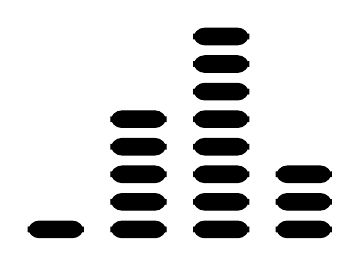
\begin{tikzpicture}[scale=0.7]
	% First Pile
	\draw[rounded corners,fill=black] (0,0) rectangle (1,0.3);
	% Second Pile
	\draw[rounded corners,fill=black] (1.5,0) rectangle (2.5,0.3);
	\draw[rounded corners,fill=black] (1.5,0.5) rectangle (2.5,0.8);
	\draw[rounded corners,fill=black] (1.5,1) rectangle (2.5,1.3);
	\draw[rounded corners,fill=black] (1.5,1.5) rectangle (2.5,1.8);
	\draw[rounded corners,fill=black] (1.5,2) rectangle (2.5,2.3);
	% Third Pile
	\draw[rounded corners,fill=black] (3,0) rectangle (4,0.3);
	\draw[rounded corners,fill=black] (3,0.5) rectangle (4,0.8);
	\draw[rounded corners,fill=black] (3,1) rectangle (4,1.3);	
	\draw[rounded corners,fill=black] (3,1.5) rectangle (4,1.8);	
	\draw[rounded corners,fill=black] (3,2) rectangle (4,2.3);	
	\draw[rounded corners,fill=black] (3,2.5) rectangle (4,2.8);	
	\draw[rounded corners,fill=black] (3,3) rectangle (4,3.3);	
	\draw[rounded corners,fill=black] (3,3.5) rectangle (4,3.8);	
	% Fourth Pile
	\draw[rounded corners,fill=black] (4.5,0) rectangle (5.5,0.3);
	\draw[rounded corners,fill=black] (4.5,0.5) rectangle (5.5,0.8);
	\draw[rounded corners,fill=black] (4.5,1) rectangle (5.5,1.3);	
	\end{tikzpicture}
	\] \pspace

\sol First, we count the number of coins in each pile: 
	\[
	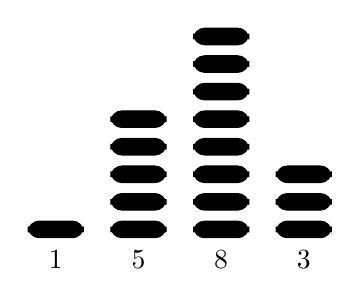
\begin{tikzpicture}[scale=0.7]
	% First Pile
	\draw[rounded corners,fill=black] (0,0) rectangle (1,0.3);
	\node at (0.5,-0.4) {$1$};
	% Second Pile
	\draw[rounded corners,fill=black] (1.5,0) rectangle (2.5,0.3);
	\draw[rounded corners,fill=black] (1.5,0.5) rectangle (2.5,0.8);
	\draw[rounded corners,fill=black] (1.5,1) rectangle (2.5,1.3);
	\draw[rounded corners,fill=black] (1.5,1.5) rectangle (2.5,1.8);
	\draw[rounded corners,fill=black] (1.5,2) rectangle (2.5,2.3);
	\node at (2,-0.4) {$5$};
	% Third Pile
	\draw[rounded corners,fill=black] (3,0) rectangle (4,0.3);
	\draw[rounded corners,fill=black] (3,0.5) rectangle (4,0.8);
	\draw[rounded corners,fill=black] (3,1) rectangle (4,1.3);	
	\draw[rounded corners,fill=black] (3,1.5) rectangle (4,1.8);	
	\draw[rounded corners,fill=black] (3,2) rectangle (4,2.3);	
	\draw[rounded corners,fill=black] (3,2.5) rectangle (4,2.8);	
	\draw[rounded corners,fill=black] (3,3) rectangle (4,3.3);	
	\draw[rounded corners,fill=black] (3,3.5) rectangle (4,3.8);	
	\node at (3.5,-0.4) {$8$};
	% Fourth Pile
	\draw[rounded corners,fill=black] (4.5,0) rectangle (5.5,0.3);
	\draw[rounded corners,fill=black] (4.5,0.5) rectangle (5.5,0.8);
	\draw[rounded corners,fill=black] (4.5,1) rectangle (5.5,1.3); 
	\node at (5,-0.4) {$3$};
	\end{tikzpicture}
	\]
We then write each of these numbers in binary. We $1= 1_2$, $5= 101_2$, $8= 1000_2$, and $3= 11_2$. We can then add these numbers in binary without carrying (adding preceding 0's for ease of reading: \par
	\begin{table}[h]
	\centering
	\begin{tabular}{rcccc}
	$1$: & $0$ & $0$ & $0$ & $1$ \\
	$5$: & $0$ & $1$ & $0$ & $1$ \\
	$8$: & $1$ & $0$ & $0$ & $0$ \\
	$3$: & $0$ & $0$ & $1$ & $1$ \\ \cline{2-5}
	        & $1$ & $1$ & $1$ & $1$
	\end{tabular}
	\end{table} \par
Because the NIM-sum is $1111 \neq 0000$, this must be an $N$-position. Therefore, the \textit{next} player to move has a winning move. Therefore, you want to go next, i.e. first. A winning move is a move which results in a NIM-sum of zero. Clearly, the 1 in the far left needs to be changed to a zero, which can only happen by removing chips from the 8-pile. We need a 1 in the remaining three columns to  result in a NUM-sum of 0 in these columns. But then we need change the 8-pile from $8= 1000_2$ to $0111_2= 7$. Therefore, the only winning move is to remove a single chip from the 8-chip pile. 



% Question 9
\newpage
\question[10] Nancy and Drew are taking out a simple discount note to pay for a cruise. This loan will be for \$3,800 for 3~months at 9.6\% yearly interest. How much do they receive from the bank? \pspace

\sol In a simple discount note, the discount (interest) is paid up-front. One then receives the maturity (loan amount) minus this discount (interest). So the amount received (the proceeds) is given by\dots
	\[
	P= M - D
	\]
where $M$ is the maturity and $D$ is the discount. We know that $D= Mrt$, where $r$ is the annual interest rate and $t$ is the time (in years). But then\dots
	\[
	D= Mrt= \$3,\!800 \cdot 0.096 \cdot \frac{3}{12}= \$91.20
	\]
Then we have\dots
	\[
	P= M - D= \$3,\!800 - \$91.20= \$3,\!708.80
	\] \pspace
Therefore, Nancy and Drew receive \$3,708.80 from the bank. 



% Question 10
\newpage
\question[10] Suppose that you invest \$7,000 into an account which earns 2.3\% annual interest, compounded quarterly. Will you have \$10,000 in the account after 6~years? Explain. If not, how long until the account contains \$10,000? \pspace

\sol The future value, $F$, of a principal amount, $P$, earning $r$ annual interest, compounded $k$ times per year for $t$ years is given by\dots
	\[
	F= P \left(1 + \dfrac{r}{k} \right)^{kt}
	\]
The principal amount is $P= \$7,\!000$. We know that $r= 0.023$ and because the interest is compounded quarterly, i.e. four times per year, $k= 4$. But then after $t= 6$~years, this investment will be worth\dots
	\[
	\begin{aligned}
	F&= P \left(1 + \dfrac{r}{k} \right)^{kt} \\[0.3cm]
	&= \$7000 \left(1 + \dfrac{0.023}{4} \right)^{4 \cdot 6} \\[0.3cm]
	&= \$7000 (1.00575)^{24} \\[0.3cm]
	&= \$7000(1.14752192) \\[0.3cm]
	&= \$8,\!032.65
	\end{aligned}
	\]
Therefore, after 6~years, the investment will only be worth \$8,032.65---not the desired \$10,000. We know the time for an investment to raise from a principal $P$ to a future value $F$ is given by $t= \frac{\log(F/P)}{k \log(1 + r/k)}$. But then\dots
	\[
	\begin{aligned}
	t&= \frac{\log(F/P)}{k \log(1 + r/k)} \\[0.3cm]
	&= \dfrac{\log(10000/7000)}{4 \log \left(1 + \frac{0.023}{4} \right)} \\[0.3cm]
	&= \dfrac{\log(1.42857143)}{4 \log(1.00575)} \\[0.3cm]
	&= \dfrac{0.35667494}{0.02293413} \\[0.3cm]
	&= 15.55 \text{ years}
	\end{aligned}
	\]
Therefore, it will take 15.55~years for the \$7,000 investment to be worth \$10,000. 


\end{questions}
\end{document}